\documentclass[pdftex,12pt,a4paper]{report}

\usepackage[pdftex]{graphicx}
\usepackage{float}
\usepackage{fancyvrb}
\fvset{xleftmargin=2em}
\usepackage{multicol}
\usepackage{wrapfig}

\usepackage{pgfplots}
\pgfplotsset{width=10cm,compat=1.9}
\usepackage{tikzscale}
\usepackage{pgfplotstable}
\usepackage{booktabs}
\usepackage[font=small,labelfont=bf,tableposition=top]{caption}

\usepackage[utf8]{inputenc} % isto é um comentário
\usepackage[portuges]{babel}
\usepackage[T1]{fontenc}
\usepackage{times}
%\usepackage{lmodern}
\usepackage[obeyspaces,spaces]{url}
\usepackage[left=25mm,right=25mm,top=25mm,bottom=25mm]{geometry}
\usepackage{titlesec}
\usepackage{mathtools}
%identa 1º paragrafo de capitulos e secções
\usepackage{indentfirst}

\newcommand{\HRule}{\rule{\linewidth}{0.5mm}}
\titleformat{\chapter}{\normalfont\huge}{\thechapter.}{20pt}{\huge}


\begin{document}

\begin{titlepage}


\begin{minipage}{0.3\textwidth}
\begin{flushleft} 

\includegraphics[width=\textwidth]{logo.png}
\end{flushleft}
\end{minipage}
\begin{minipage}{0.6\textwidth}
\begin{flushright} 

\textsc{Departamento de Engenharia Informática}\\[0.1cm]
\bfseries Mestrado Integrado em Engenharia Informática \\ [0.1cm]
\bfseries \textit{Programação Orientada aos Objetos}\\[8mm]

\end{flushright}
\end{minipage}


\vspace{3cm}


\begin{center}


\LARGE UMeR

\Large \textbf{\textit{Serviço de transporte de passageiros}}\\[1.5cm]


{\Large \bfseries Grupo XX\\[2cm] }


\noindent\begin{minipage}[b]{.2\textwidth}
	
\includegraphics[scale=0.18]{celia}
	\small{Célia Figueiredo a67637}
\end{minipage} 
\hfill
\begin{minipage}[b]{.2\textwidth}
	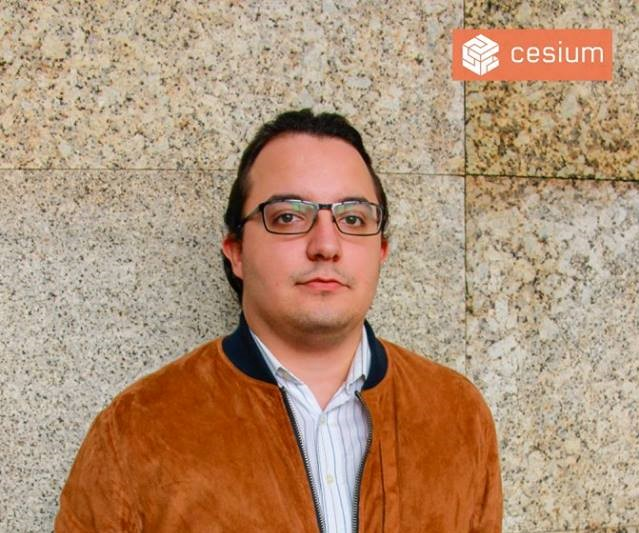
\includegraphics[scale=0.3]{luis}
	\small{José Carlos Faria a67638}
\end{minipage}
\hfill
\begin{minipage}[b]{.2\textwidth}
	
\includegraphics[scale=0.63]{nelson}
	\small{Márcia Costa a67672}
\end{minipage}




\vspace{3ex}


\vfill

\large Braga, {\large \today}

\end{center}
\end{titlepage}


\tableofcontents

\begin{abstract}

O presente relatório descreve o trabalho efetuado para a realização do projeto, onde foi pedido a implementação de um serviço de transporte de passageiros (UMeR) com o uso da linguagem \textit{JAVA} esta que é orientada aos objetos. 

\end{abstract}
\chapter{Introdução}
\label{cap:intro}

No âmbito da Unidade Curricular de Programação Orientada aos Objectos pertencente ao plano de estudos do 2º ano do Mestrado Integrado em Engenharia Informática foi proposto o desenvolvimento de um serviço de transporte de passageiros. 



%\chapter{Descrição geral do projeto}
\section{UMeR}
Pretende-se que a aplicação a ser desenvolvida dê suporte a toda a funcionalidade que permita que um utilizador realize uma viagem num dos táxis da \textbf{UMeR}. O processo deve abranger todos os mecanismos de criação de utilizadores, motoristas, automóveis e posteriormente a marcação das viagens, a realização das mesmas e respectiva imputação do preço. Pretende-se também que o sistema guarde registo de todas as operações efectuadas e que depois tenha mecanismos para as disponibilizar (exemplo: viagens de um utilizador, extracto de viagens de um taxi num determinado período, valor facturado por um taxi num determinado período, etc.). 

Cada perfil de utilizador deve apenas conseguir aceder às informações e funcionalidades respectivas.

\begin{itemize}
	\item Os clientes dos táxis UMeR poderão:
	\begin{enumerate}
		\item solicitar uma viagem ao táxi mais próximo das suas coordenadas;
		\item solicitar uma viagem a um táxi específico;
		\item fazer uma reserva para um táxi específico que, de momento, não está disponível.
	\end{enumerate}
\end{itemize}

\begin{itemize}
	\item Os motoristas poderão:
	\begin{enumerate}
		\item sinalizar que estão disponíveis para serem requisitados;
		\item registar uma viagem para um determinado cliente;
		\item registar o preço que custou determinada viagem.
	\end{enumerate}
\end{itemize}

\subsection{Actores do sistema}

Existirão dois tipos distintos de actores no sistema, que partilham a seguinte informação:
\begin{itemize}
	\item email (que identifica o utilizador);
	\item nome;
	\item password;
	\item morada;
	\item data de nascimento.
\end{itemize}

\subsubsection{Cliente}
O Cliente representa a pessoa que solicita e efectua uma viagem de táxi. O cliente está sempre numa determinada localização (expressa em x e y, isto é, num espaço 2D) e escolhe um táxi específico ou então solicita o táxi mais perto que esteja disponível. O cliente tem também uma relação de todas as viagens que fez, com toda a informação relativa à viagem.

\subsubsection{Motorista - colaborador da UMeR}
O motorista conduz o táxi e além da informação atrás referida tem também dados relativos a: 
\begin{itemize}
	\item grau de cumprimento de horário estabelecido com o cliente, dado por um factor entre 0 e 100;
	\item classificação do motorista, dado numa escala de 0 a 100, calculada com base na classificação dada pelo cliente no final da viagem;
	\item histórico das viagens realizadas;
	\item número de kms já realizados na UMeR;
	\item informação sobre se está ou não disponível em determindado momento, isto é, se está ou não a trabalhar.
\end{itemize}

\subsection{Os táxis UMeR}

O ecossistema do UMeR contempla diferentes tipos de viaturas de aluguer (táxis). Neste momento estão em funcionamento os seguintes tipos de viaturas:

\begin{itemize}
	\item carros ligeiros;
	\item carrinhas de nove lugares;
	\item motos.
\end{itemize}
Cada um destes tipos de viaturas tem associada:
\begin{itemize}
	\item uma velocidade média por km;
	\item um preço base por km;
	\item um factor de fiabilidade, que determina a capacidade da viatura cumprir o tempo acordado com o cliente. Sempre que se realiza uma viagem é calculado (através da invocação de um random()) a capacidade de o veículo cumprir com o tempo acordado com o cliente. Este factor tem um efeito multiplicador sobre o tempo fornecido ao cliente.
\end{itemize}

Existem ainda alguns tipos de viaturas que possibilitam a existência de uma fila de espera de marcações. Quando o táxi não está disponível (por exemplo, pelo facto do condutor estar fora do horário de trabalho) é possível para essas viaturas aceitarem reservas de clientes. As reservas serão satisfeitas por ordem de chegada. Uma viatura sabe sempre a localização (em x e y) onde está. Quando realiza um serviço desloca-se para as coordenadas indicadas pelo cliente e fica aí parado até que seja solicitado um novo serviço.

\subsection{Fazer uma viagem no UMeR}
O processo de fazer uma viagem no UMeR segue as seguintes regras:
\begin{enumerate}
	\item o cliente indica as coordenadas x e y em que se encontra;
	\item o cliente decide se pretende chamar um táxi específico ou então solicitar o que está mais próximo;
	\item por uma questão de simplificação, os UMeR deslocam-se sempre em linha recta pelo que o cálculo da distância entre o cliente e o táxi é feito pela cálculo da distância euclidiana (exemplo: se o cliente estiver em (0,0) e o táxi em (2,2) a distância é de 2.8284 kms);
	\item após ser calculada a distância consegue-se saber, dadas as características do táxi, quanto tempo demora a chegar ao cliente e depois ao destino que o cliente solicita;
	\item o táxi indica ao cliente qual o custo estimado da viagem, tendo em conta o deslocamento que é necessário efectuar, e o tempo total de viagem;
	\item de acordo com a fiabilidade do carro (e de outros factores que pode considerar: a destreza do condutor, as condições metereológicas, etc.) é calculado o tempo real da viagem. Se a diferença for superior a 25\% do tempo estimado, então o preço a cobrar é o combinado com o cliente. Se a diferença for igual ou inferior a 25\% o valor é ajustado para o valor real em função do tempo decorrido;
	\item o táxi fica no ponto definido como fim da viagem à espera de nova solicitação de serviço;
	\item após a viagem o cliente pode dar uma nota ao motorista e fica com o documento relativo à viagem guardado na sua área pessoal.
\end{enumerate}

\subsection{Motoristas individuais vs Empresas de Táxi}
Numa primeira fase o UMeR foi pensado para condutores que conduziam a sua viatura e fazem serviço de transporte de clientes. No entanto, e devido ao sucesso do negócio, foram criadas empresas que possuem várias viaturas (em teoria de diversos tipos) e que empregam vários motoristas. A gestão que é feita destas empresas implica que após a criação da empresa se possam adicionar viaturas e motoristas, e que uma mesma viatura possa ser conduzida por motoristas diferentes (em tempos diferentes).

\subsection{Viaturas com Fila de Espera}
O UMeR possibilita que algumas viaturas possam ser definidas como possuindo uma fila de espera, que possibilita que quando a viatura está indisponível os pedidos sejam adicionados a uma fila de espera. Quando o veículo fica disponível são executadas todas as viagens inseridas na fila de espera, pela ordem de chegada. Os veículos com fila de espera possibilitam este comportamento, sendo que os demais não exibem este comportamento e nessa situação se a viatura estiver indisponível não será candidata a efectuar viagens.

\chapter{Arquitetura das Classes}
Neste capítulo falaremos do esqueleto da  aplicação UMeR, serão abordadas as classes presentes na aplicação assim como os atributos e funcionamento de cada uma e também as decisões tomadas.
\begin{figure}[htb]
	\centering
	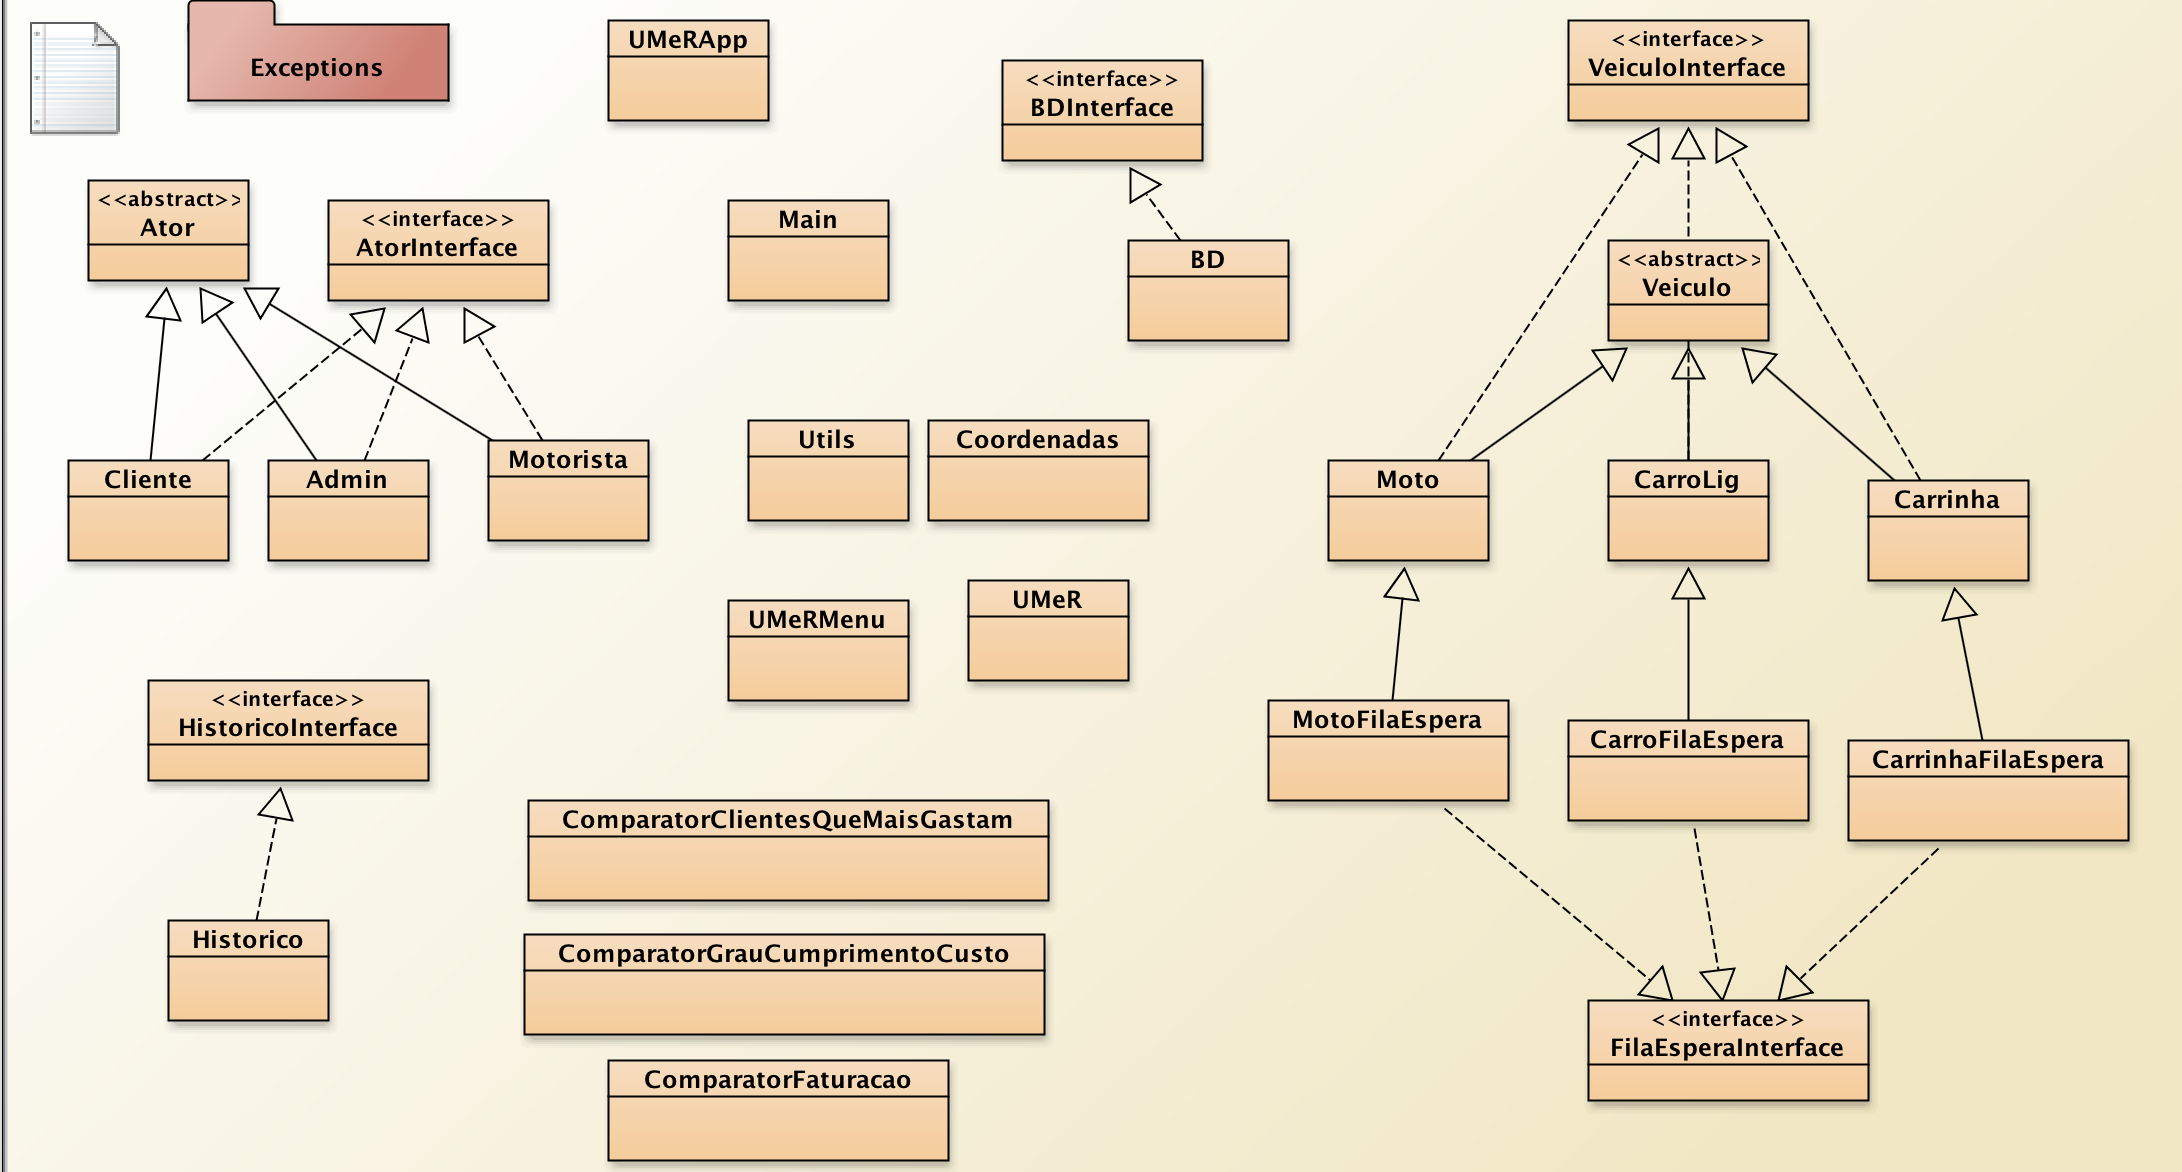
\includegraphics[scale=0.45]{imagem/esquemaClasses}
	\caption{Esquema de Classes do BlueJ }
	\label{p2:fig:p2_classes}
\end{figure}

\newpage

\section{AtorInterface}
A interface AtorInterface define todos os métodos que os utilizadores da aplicação deverão ter definidos. 
Se no futuro for pretendido adicionar novos tipos de atores ao sistema, essas classes deverão também elas implementar esta interface.  Desta forma poder-se-á inserir novos tipos de utilizadores à base de dados sem dificuldades. Como se pode visualizar na base de dados os utilizadores (motoristas, clientes e admins ) são coleções do tipo AtorInterface. Pode-se portanto adicionar os novos tipos de atores a cada uma destas coleções. 
 

\subsection{ Ator}
A classe  \textit{Ator} é uma classe abstrata e sevirá  como “modelo” para outras classes que dela herdem, não podendo ser instanciada por si só. Para ter um objeto de uma classe abstrata é necessário criar uma classe mais especializada que herda dela e então instanciar essa nova classe. Neste caso foram criadas as classes \textit{Admin}, \textit{Cliente} e  \textit{Motorista} que herdam a informação que está na classe superior (Ator).

\begin{figure}[htpb]
	\centering
	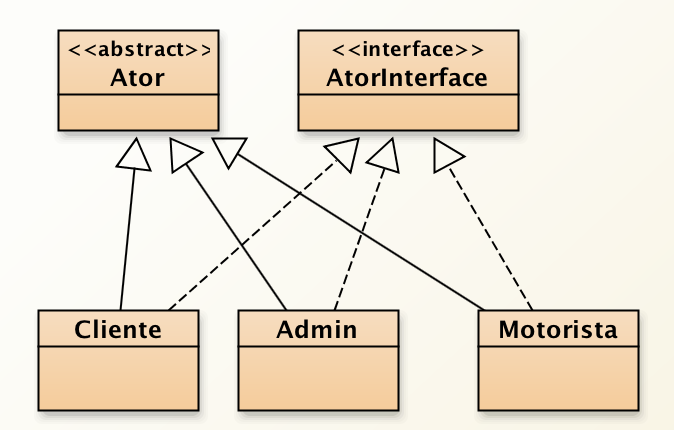
\includegraphics[scale=0.6]{imagem/atores}
	\caption{Classes }
	\label{p2:fig:p2_atoresr}
\end{figure}

As variáveis de instância da classe abstrata \textit{Ator} são apresentadas de seguida: 
\begin{verbatim}
private String email; 
private String nome; 
private String password; 
private String morada; 
private LocalDate dataNascimento; 
\end{verbatim}


\subsection{Admin}

Na classe \textit{Admin} estarão todos os dados herdados da classe \textit{Ator}. 


\subsection{Cliente}
Na classe \textit{Cliente} estarão todos os dados herdados da classe \textit{Ator}. 

\begin{verbatim}
private Coordenadas loc; //localização atual do cliente
private boolean emViagem;
\end{verbatim}
\subsection{Motorista}
Na classe \textit{Motorista} estarão todos os dados herdados da classe \textit{Ator}. 

\begin{verbatim}
private int grauCumprimentoHorario; //0-100
private int classificacao; //0-100
private double totalKms; 
private boolean disponivel;//verifica se está disponivel ou não 
private boolean horarioTrabalho; //verificar se está no horário de trabalho
private double destreza; //valor entre 0.5 e 1.9
private VeiculoInterface veiculo; 
private Historico viagemEmProcesso;
private int totalViagens;
\end{verbatim}

Decidimos que a destreza do motorista seria atribuida através da invocação de um random() que gera valores entre 0,5  e 1,9 afim de gerar alguma aleatoriedade nos tempos obtidos das viagens efetuadas. 
\begin{verbatim}
this.destreza = Utils.generateRandom(0.5f, 1.9f); 
\end{verbatim}

\newpage
\section{VeiculoInterface}

A interface VeiculoInterface define todos os métodos que os veiculos da aplicação deverão ter definidos. 
Se no futuro for pretendido adicionar novos tipos de veiculos ao sistema, essas classes deverão também elas implementar esta interface.  Desta forma poder-se-á inserir novos tipos de veiculosd à base de dados sem dificuldades. Como se pode visualizar na base de dados os veiculos (carros, motos, carrinhas, etc ) são coleções do tipo VeiculoInterface. Pode-se portanto adicionar os novos tipos de veiculos à coleção. 


\begin{figure}[htpb]
	\centering
	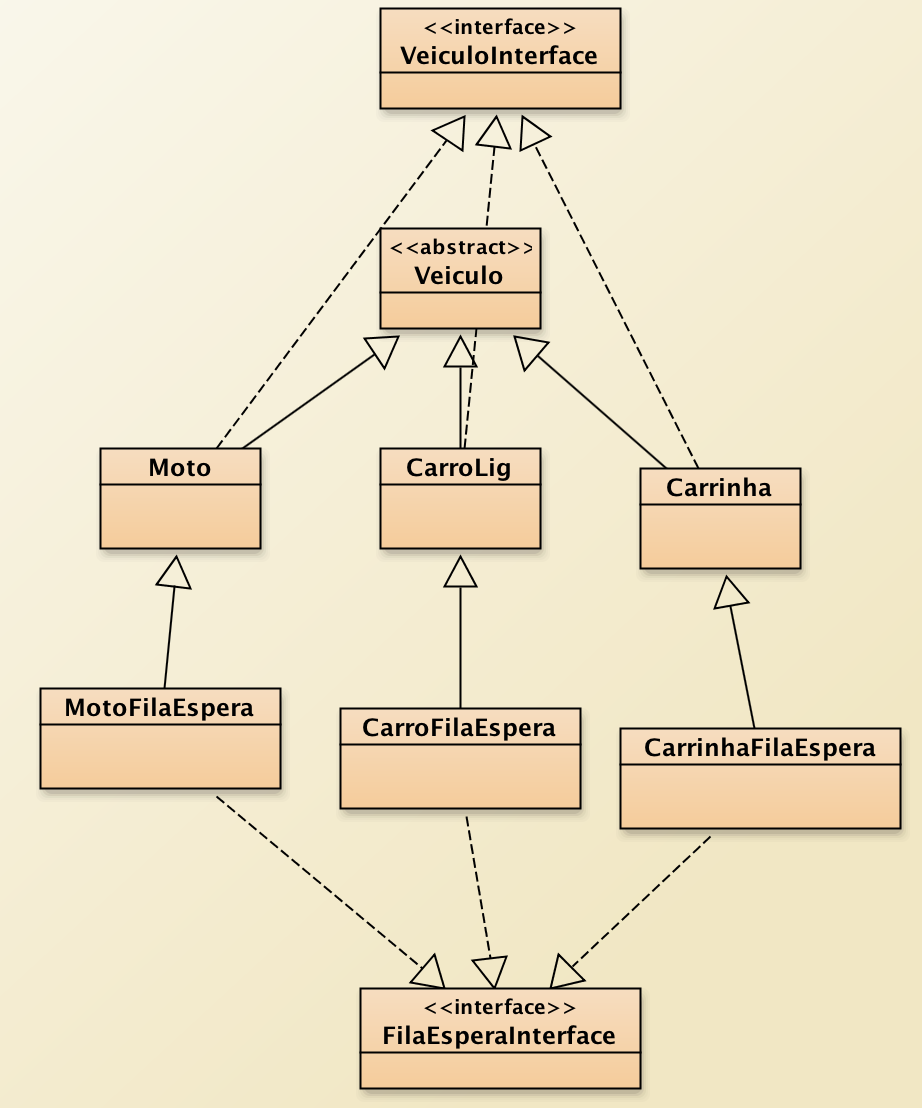
\includegraphics[scale=0.6]{imagem/veiculo}
	\caption{Classes }
	\label{p2:fig:p2_veiculos}
\end{figure}

\subsection{Veiculo}

\begin{verbatim}
private String matricula; 
private String marca; //Acrescentou-se a variável de instância marca, 
para o cliente poder escolher um carro com base na marca do veiculo

private float fiabilidade;//0 a 2 randon()
private Coordenadas loc;
\end{verbatim}

\section{Moto}
\begin{verbatim}
private static final int lugaresLivres = 1;
private static final double vm = 40.5; 
private static final double precoPorKm = 2.1;
\end{verbatim}

\subsection{MotoFilaEspera}
\begin{verbatim}
private List<Cliente> filaClientes;
\end{verbatim}

\section{CarroLig}

\begin{verbatim}
 private static final int lugaresLivres = 4;
private static final double vm = 65; 
private static final double precoPorKm = 3.5;
\end{verbatim}

\subsection{CarroFilaEspera}
\begin{verbatim}
private List<Cliente> filaClientes;
\end{verbatim}

\section{Carrinha}

\begin{verbatim}
private static int lugaresLivres = 8;
private static final double vm = 55;
private static final double precoPorKm = 5.1;
\end{verbatim}

\subsection{CarrinhaFilaEspera}
\begin{verbatim}
private List<Cliente> filaClientes;
\end{verbatim}

\newpage
\section{HistoricoInterface}
A interface HistoricoInterface define todos os métodos que os históricos da aplicação deverão ter definidos. 
Se no futuro for pretendido adicionar novos tipos de históricos ao sistema, essas classes deverão também elas implementar esta interface.  Desta forma poder-se-á inserir novos tipos de históricos à base de dados sem dificuldades. Como se pode visualizar na base de dados os históricos são coleções do tipo HistoricoInterface. Pode-se portanto adicionar os novos tipos de históricos à coleção. 

\subsection{Historico}
\begin{figure}[htpb]
	\centering
	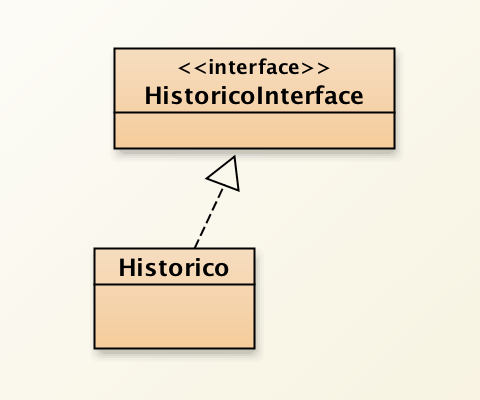
\includegraphics[scale=0.6]{imagem/historico}
	\caption{Classes }
	\label{p2:fig:p2_historico}
\end{figure}
\begin{verbatim}
private String emailCliente; 
private String emailMotorista; 
private LocalDateTime dataDeInicioDeServico;
private double distancia;
private double tempoEstimado; 
private double tempoReal;
private double valorEstimado; 
private double valorCobrado; 
private String estadoTempo;
private String estadoTransito; 
private boolean terminado; 
private Coordenadas origem;
private Coordenadas destino;
private int classificacao;
\end{verbatim}

\section{Utils}
Adicionalmente a classe \textit{Utils} tem implementado um método que encripta a password. E um método que gera números random com intervalos de 0.1. 

\subsection{Meteorologia}

Esta classe é usada para gerar fatores de aleatoriedade no cálculo real do tempo de viagem.

\begin{verbatim}
public static final String sol = "Sol"; 
public static final String nevoeiro  = "Nevoeiro"; 
public static final String granizo = "Granizo";
public static final String chuva = "Chuva";
public static final String neve = "Neve"; 
\end{verbatim}

\subsection{Trânsito}

Esta classe é usada para gerar fatores de aleatoriedade no cálculo real do tempo de viagem.

\begin{verbatim}
public static final String st = "Sem Transito"; 
public static final String tn = "Transito Normal"; 
public static final String mt  = "Muito Transito"; 
\end{verbatim}

\section{Coordenadas}

Esta classe guarda a localização de um utilizador. O construtor vazio está a ser usado na aplicação para gerar localizações aleatórias quando se criam os utilizadores. 

\begin{verbatim}
private double x;
private double y;
\end{verbatim}

As cordenadas também são iniciadas com o método random(). 
\begin{verbatim}
this.x=Utils.generateRandom(0f, 100f);
this.y=Utils.generateRandom(0f, 100f);
\end{verbatim}

O método getDistancia() calcula a distancia euclidiana, este será um método importante na execução da simulação de uma viagem. 
\begin{verbatim}
public double getDistancia (Coordenadas c){
    double distancia=0; 
    distancia = Math.sqrt( Math.pow((this.x - c.getX()),2 ) +
                           Math.pow((this.y - c.getY()),2 ));
    return distancia; 
}
\end{verbatim}

\section{BDInterface}
A interface BDInterface define todos os métodos que as classes que geram dados da aplicação deverão ter definidos. 

Se no futuro se pretender guardar a informação numa base de dados (Oracle por exemplo), esta classe deverá implementar a BDInterface. Desta forma, a mudança de classes que geram os dados guardados é muito simples uma vez que o resto da aplicação continuará a usar os mesmos métodos(definidos na BDInterface) que usa neste momento independentemente da forma como a classe implementa os métodos definidos pela interface. 

\subsection{BD}

As coleções clientes, motoristas e admins são do tipo Map e estão organizados pela chave que é o respetivo email. Uma vez que se efetuam muitas pesquisas, sobre estes dados com a chave email, a melhor opção seria um HashMap uma vez que a pesquisa pela chave é instântanea. 

Para a coleção de veiculos foi utilizada também um HashMap em que a chave é a matricula e os motivos são os mesmso descritos em cima.  Apesar de neste momento não se efetuar muitas pesquisas pela chave, imagina-se que no futuro tal poderá acontecer. 

A colecção de históricos escolhida foi o Set, pois não devem ser permitidos históricos repetidos. Uma vez que algumas das funcionalidades da aplicação implicavam percorrer os dados por ordem (data), pareceu-nos indicado usar um TreeSet e desta forma ter os dados guardados e ordenados de forma a facilitar as funcionalidade do programa.  

\begin{verbatim}
private Map<String, AtorInterface> clientes;
private Map<String, AtorInterface> motoristas; 
private Map<String, AtorInterface> admins; 
private Map<String,VeiculoInterface> veiculos; 
private Set<Historico> historico;
\end{verbatim}

\section{UMeRMenu}

Esta classe tem como objetivo facilitar a criação de menus e a leitura da opção introduzida. 

\begin{verbatim}
private String titulo;
private List<String> opcoes;
private int op;
\end{verbatim}

\section{UMeR}

Esta classe é o coração da aplicação, uma vez que é nela que está centralizada a lógica das gestão de viagens. É nesta classe que estão definidos os métodos para o calculo do tempo real, estimado, custo real e estimado, bem como métodos para devolver o motorista mais perto e estatisticas da aplicação. Sempre que necessário a UMeR delega a gestão dos dados(ler, guardar, atualizar, apagar) na classe da base de dados (BDInterface). 
Após login efetuado com sucesso a variável de instância atorloggado é inicializada com o utilizador que acabou de iniciar sessão. É com base nesta variável que a interface da aplicação(UMeRApp) decide quais os menus a apresentar.  

\begin{verbatim}
private BDInterface baseDeDados;
private AtorInterface atorLoggado;
private int tentativasDeLoginFalhadas;
\end{verbatim}

\section{UMeRApp}

Esta classe é responsável pela interface da aplicação. 

\begin{verbatim}
private static UMeR umer;
private static UMeRMenu menu_principal;
private static UMeRMenu menu_registar_atores;
private static UMeRMenu menu_motorista;
private static UMeRMenu menu_cliente;
private static UMeRMenu menu_dados_pessoais;
private static UMeRMenu menu_cliente_efetuarViagem;
private static UMeRMenu menu_admin;
private static UMeRMenu menu_registar_veiculos;
private static UMeRMenu menu_solicitarViagem; 
private static UMeRMenu menu_inserir_coord_destino;
private static UMeRMenu menu_terminar_viagem; 
private static UMeRMenu menu_terminar_horario_trabalho;
private static UMeRMenu menu_iniciar_horario_trabalho;
private static UMeRMenu menu_proposta_viagem;
private static UMeRMenu menu_historico;
\end{verbatim}





\chapter{Funcionamento da Aplicação UMeR}
\section{Menu Inicial}
Esta é  uma aplicação com uma interface para o utilizador muito simples, foi pensada
de maneira a que o utilizador pudesse tirar o maior proveito da mesma, com comandos simples, tendo em conta que todos os menus funcionam à base de opções por números.
Quando um utilizador executa a aplicação o primeiro menu a que está sujeito é o
seguinte:

\begin{figure}[htpb]
\centering
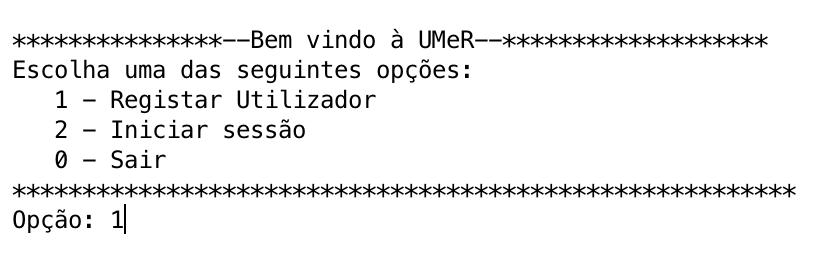
\includegraphics[scale=0.6]{imagem/menuInicial}
\caption{Menu Inicial  }
\label{p3:fig:p2_paginicial}
\end{figure}

\section{Menu Inicial-Registo}

O utilizador consoante o seu tipo poderá efetuar um registo na aplicação. Será apresentado o seguinte menu para o registo de atores no sistema: 

\begin{figure}[htpb]
	\centering
	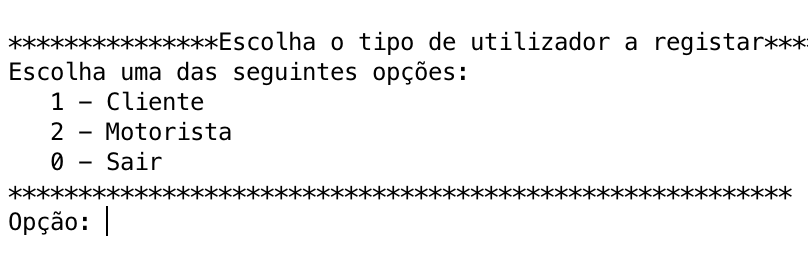
\includegraphics[scale=0.6]{imagem/escolhaTipoAtor}
	\caption{Menu de Registo na Aplicação }
	\label{p3:fig:p2_escolhaTipoAtor}
\end{figure}
Os dados pedidos no ato de registo quer de clientes ou motoristas é o mesmo, no entanto serão guardados de acordo com o tipo inicialmente escolhido. 
\newline

\noindent\begin{minipage}[b]{.4\textwidth}
	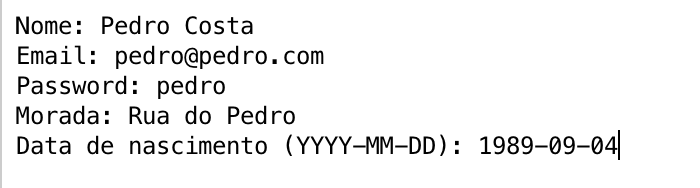
\includegraphics[scale=0.6]{imagem/exemploregistomotorista}
	\small{Exemplo de registo de um motorista}
\end{minipage} 
\hfill
\begin{minipage}[b]{.4\textwidth}
	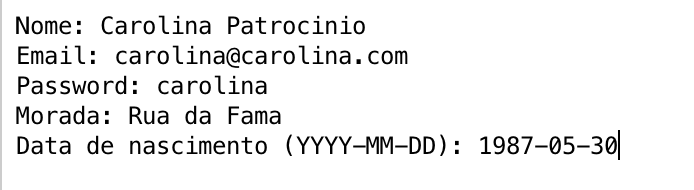
\includegraphics[scale=0.6]{imagem/exemploderegistocliente}
	\small{Exemplo de registo de um cliente}
\end{minipage}
\hfill

\section{Menu Inicial - Iniciar Sessão }
\subsection{Funcionalidades de Cliente}
O Cliente tem à sua disposição várias funcionalidades tais como: Soliciar uma viagem; Visualizar o histórico de viagens; Classificar viagens e ainda Ver e Editar dados pessoais. 
\begin{figure}[htpb]
	\centering
	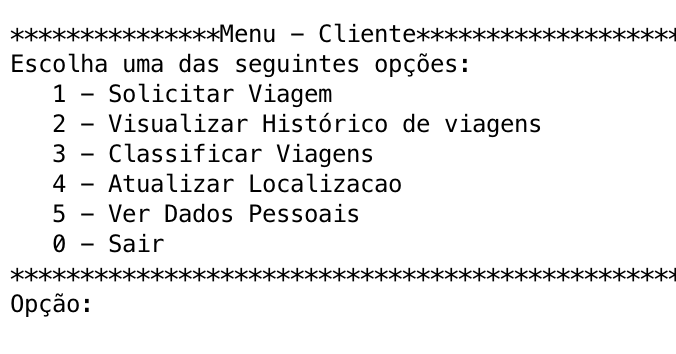
\includegraphics[scale=0.7]{imagem/menuCliente}
	\caption{Menu de Cliente }
	\label{p3:fig:p3_menuCliente}
\end{figure}

\begin{enumerate}
	\item \textbf{Solicitar Viagem}

Ao escolher "Solicitar Viagem" será pedido ao Cliente para introduzir as Coordenadas de destino. Após a inserção das Coordenadas é pedido ao Cliente para escolher se quer o táxi que se encontra mais próximo dele ou se prefere escolher um táxi especifico. 

\noindent\begin{minipage}[b]{.5\textwidth}
	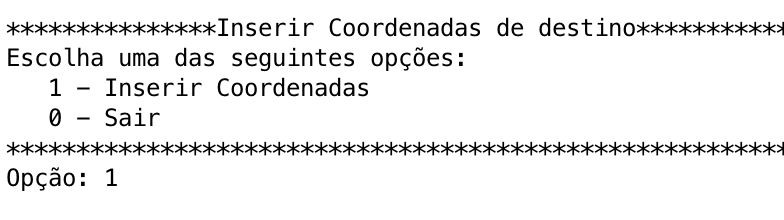
\includegraphics[scale=0.55]{imagem/inserirDestino}
	\small{Menu para inserir as coordenadas}
\end{minipage} 
\hfill
\begin{minipage}[b]{.45\textwidth}
	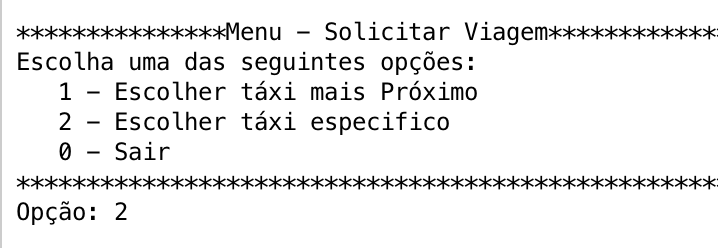
\includegraphics[scale=0.55]{imagem/coorInseridas}
	\small{Menu após a inserção de coordenadas: Escolha de táxi}
\end{minipage}
\hfill

Ao Cliente após escolher a opção 1, é-lhe apresentado um menu com os dados do táxi que se encontra mais perto da localização do cliente. De seguida é dada a opção de aceitar fazer a viagem ou não. 

\noindent\begin{minipage}[b]{.4\textwidth}
	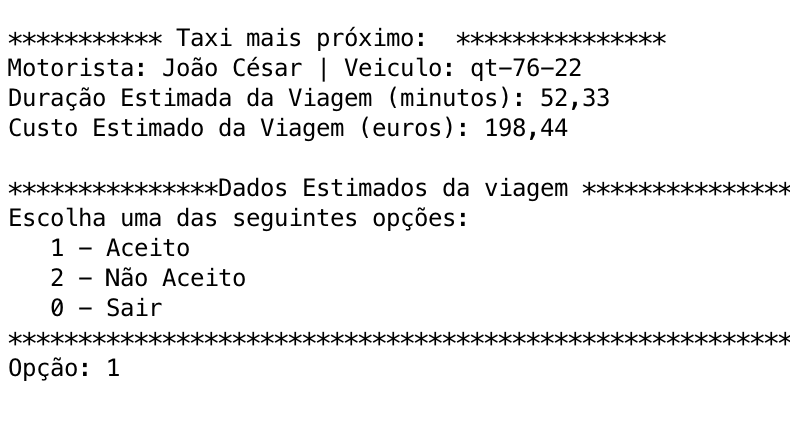
\includegraphics[scale=0.4]{imagem/taxiMaisProx}
	\small{Menu com os dados do taxi mais próximo}
\end{minipage} 
\hfill
\begin{minipage}[b]{.45\textwidth}
	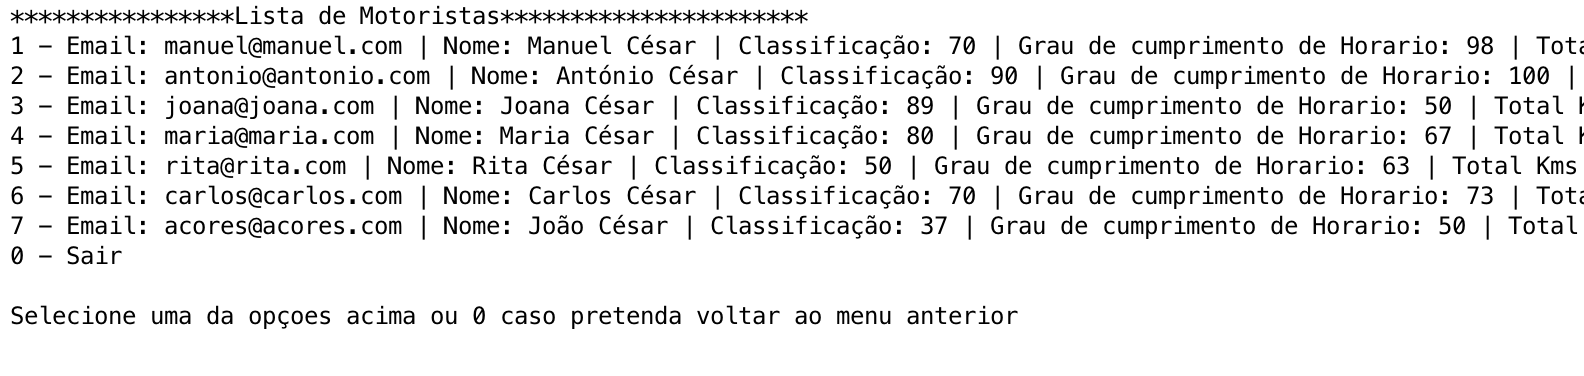
\includegraphics[scale=0.35]{imagem/escolherTaxiEspecifico}
	\small{Menu com os dados dos táxis disponiveis}
\end{minipage}
\hfill

\newpage
Se aceitar fazer a viagem aparecer-lhe-á o seguinte menu, com a informação do tempo que o táxi demorará até chegar à localização do cliente. 

\begin{figure}[htpb]
	\centering
	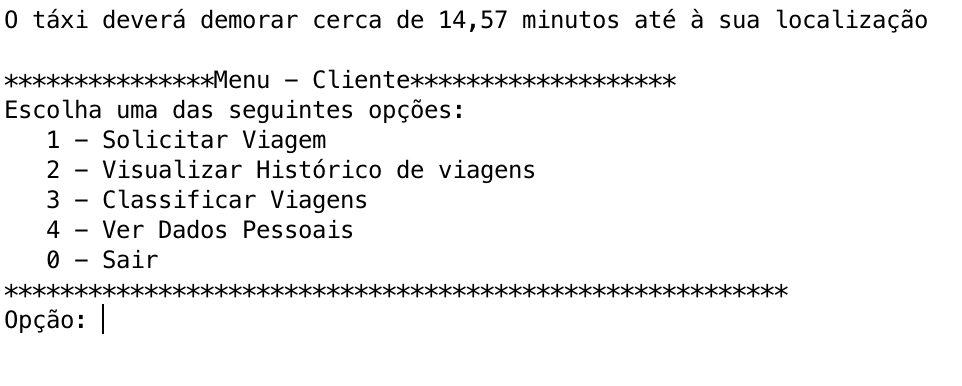
\includegraphics[scale=0.6]{imagem/aceitarViagem}
	\caption{Menu de Viagem aceite }
	\label{p3:fig:p3_aceitarViagem}
\end{figure}

Caso o cliente tenha efetuado uma viagem e esta ainda estiver a decorer, não poderá solicitar outra viagem sem que a atual tenha terminado. Será mostrada uma mensagem como a seguinte: 
\begin{figure}[htpb]
	\centering
	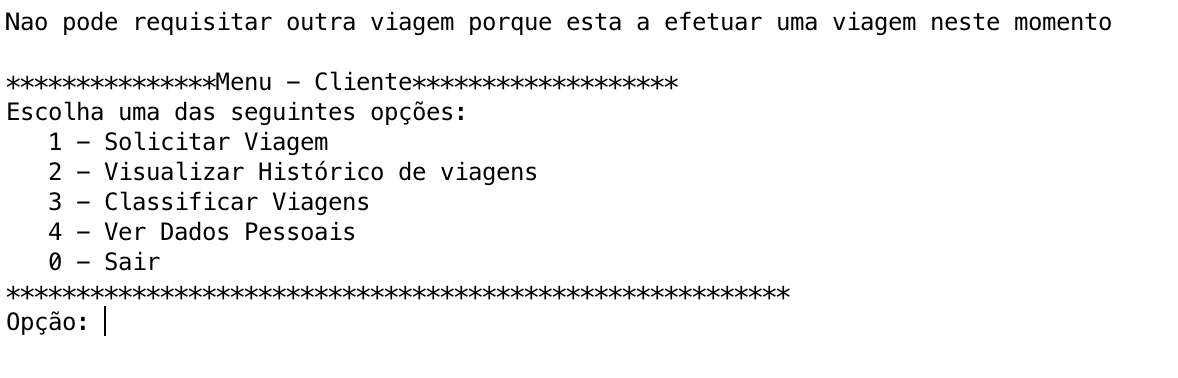
\includegraphics[scale=0.6]{imagem/erroEmViagem}
	\caption{Menu de Erro: Cliente está em viagem }
	\label{p3:fig:p3_erroEmViagem}
\end{figure}


\item \textbf{Visualizar Histórico de viagens }

O Cliente poderá visualizar o seu histórico de todas viagens efetuadas e poderá escolher como quer ver a informação ou entre datas ou todas as viagens. 

\noindent\begin{minipage}[b]{.3\textwidth}
	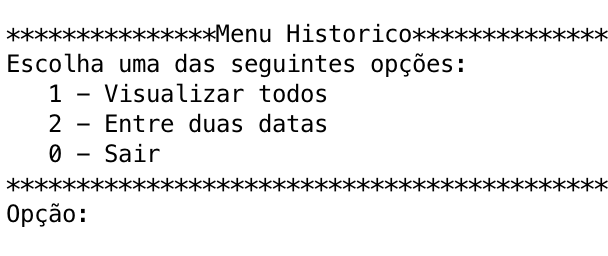
\includegraphics[scale=0.4]{imagem/menuHistorico}
	\small{Menu para escolher como visualizar histórico}
\end{minipage} 
\hfill
\begin{minipage}[b]{.45\textwidth}
	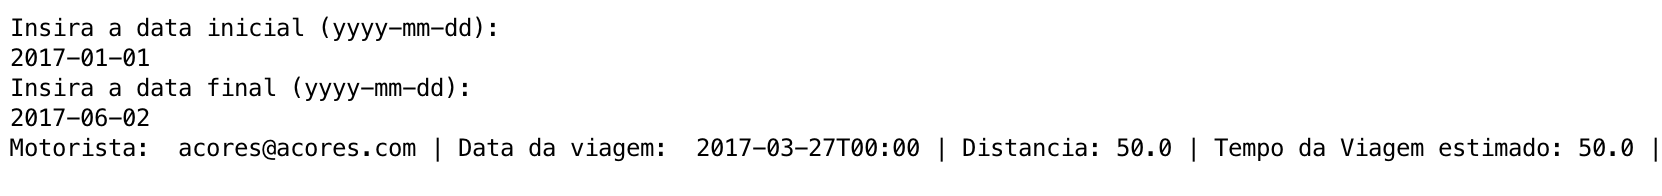
\includegraphics[scale=0.4]{imagem/verHistoricoEntreDatas}
	\small{Menu ver histórico entre datas}
\end{minipage}
\hfill


\newpage
\item \textbf{Classificar Viagens} 

O menu para classificação de viagem, servirá para o cálculo da média de classificação geral do Motorista. 

\noindent\begin{minipage}[b]{.4\textwidth}
	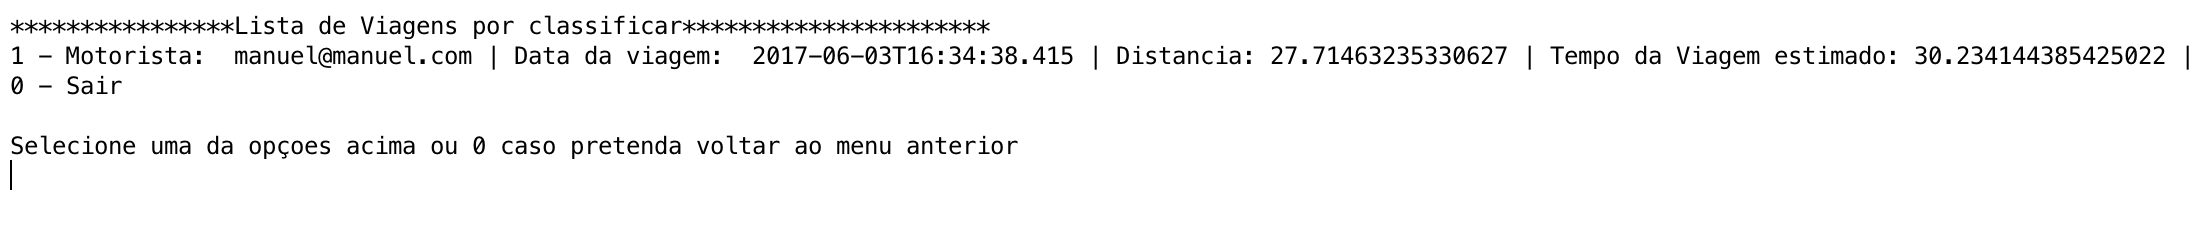
\includegraphics[scale=0.3]{imagem/listaViagensPorClassificar}
	\small{Menu para Cliente classificar a viagem }
\end{minipage} 
\hfill
\begin{minipage}[b]{.4\textwidth}
	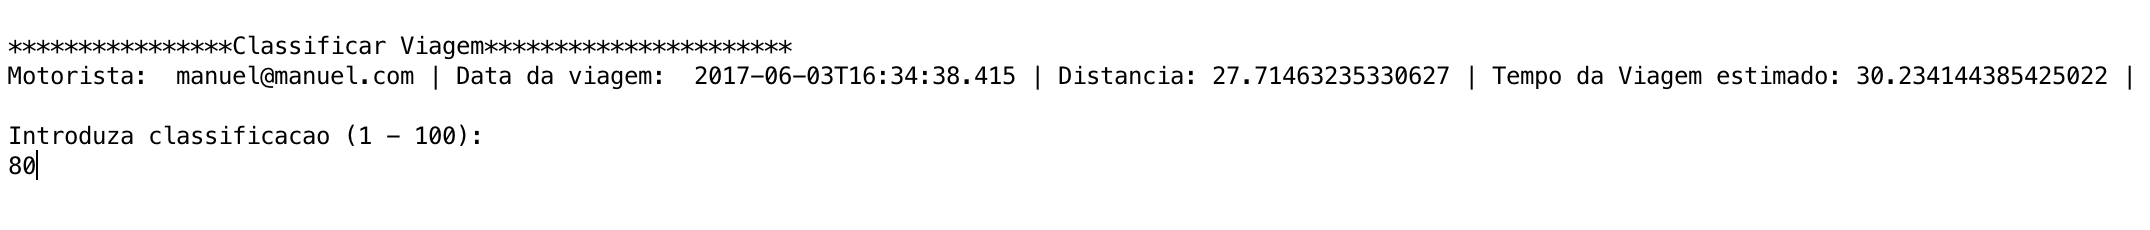
\includegraphics[scale=0.4]{imagem/classificarViagem}
	\small{Menu para classificação da viagem}
\end{minipage}
\hfill


\item \textbf{Atualizar Localização} 

O menu para atualizar localização serve para o cliente após fazer uma viagem, atualizar para uma nova localização em que se encontra para efetuar uma nova viagem. 

\begin{figure}[htpb]
	\centering
	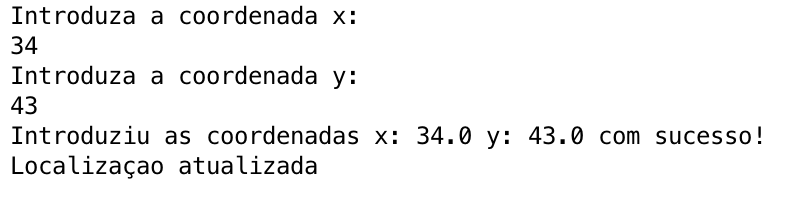
\includegraphics[scale=0.6]{imagem/atualizarLocalizacao}
	\caption{Atualizar Localização}
	\label{p3:fig:p3_atualizarLocalizacao}
\end{figure}



\item \textbf{Ver dados pessoais }

É oferecida aos Clientes e a todos os outros utilizadores a possibilidade de verem os seus dados e editarem todos os campos com a excepção do email. 
\begin{figure}[htpb]
	\centering
	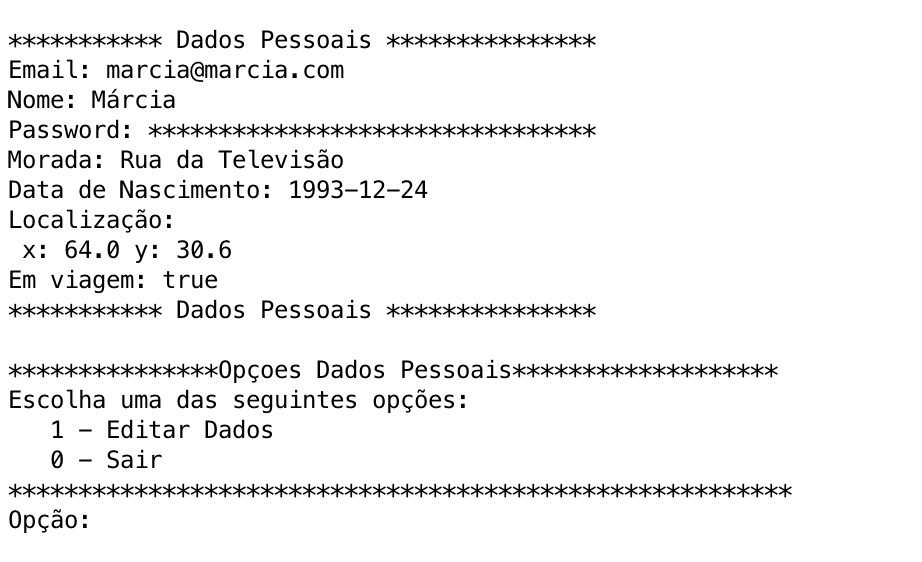
\includegraphics[scale=0.6]{imagem/verDadosPessoais}
	\caption{Menu de visualização e edição dos dados Pessoais }
	\label{p3:fig:p3_verDadosPessoais}
\end{figure}

\end{enumerate}


\newpage
\subsection{Funcionalidades de Motorista}
O motorista na UMeR poderá registar e remover o seu veiculo, gerir viagens é para iniciar uma viagem que esteja pendente; gerir horário de trabalho serve para não aceitar viagens quando não está a trabalhar. Poderá ver o histórico das viagens efetuadas, quais os seus melhores 10 clientes e ver e editar os seus dados pessoais. O menu apresentado será o seguinte: 
\begin{figure}[htpb]
	\centering
	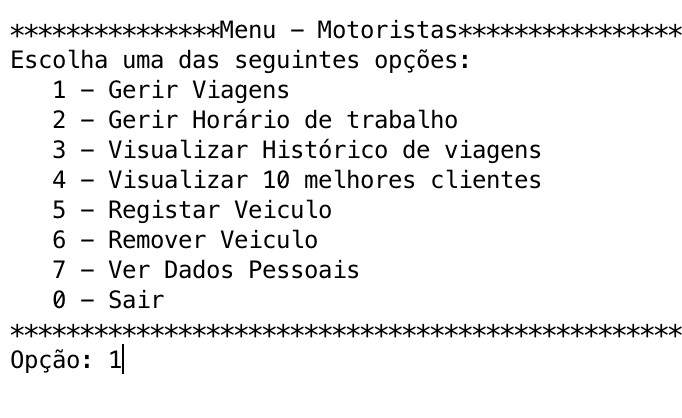
\includegraphics[scale=0.6]{imagem/menuMotorista}
	\caption{Menu de Motorista }
	\label{p3:fig:p3_menuMotorista}
\end{figure}

\begin{enumerate}
	\item \textbf{Gerir Viagens}

Após escolher gerir uma viagem será apresentado o menu com a opção de terminar viagem, caso  Ao efetuar este passo o motorista passa a estar num disponivel, isto é fica apto para receber novas viagens. 

\hfill
\noindent\begin{minipage}[b]{.4\textwidth}
	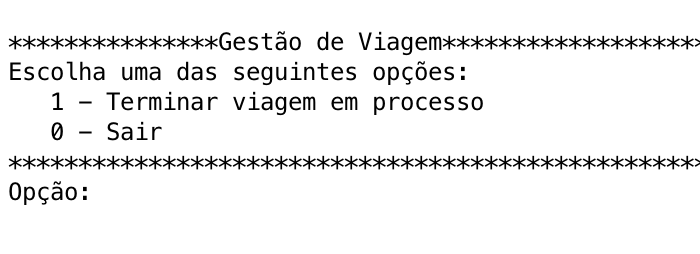
\includegraphics[scale=0.55]{imagem/gerirViagem}
	\small{Menu do motorista para terminar uma viagem}
\end{minipage} 
\hfill
\begin{minipage}[b]{.4\textwidth}
	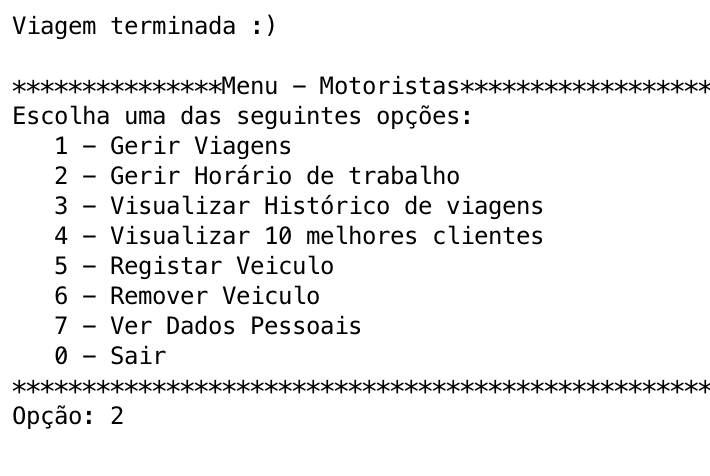
\includegraphics[scale=0.5]{imagem/viagemTerminada}
	\small{Menu após terminar viagem}
\end{minipage}
\hfill 

\item \textbf{Gerir Horário de trabalho}

Na opção de gerir horário de trabalho é apresentado o seguinte menu em que o motorista o poderá terminar. 

\noindent\begin{minipage}[b]{.4\textwidth}
	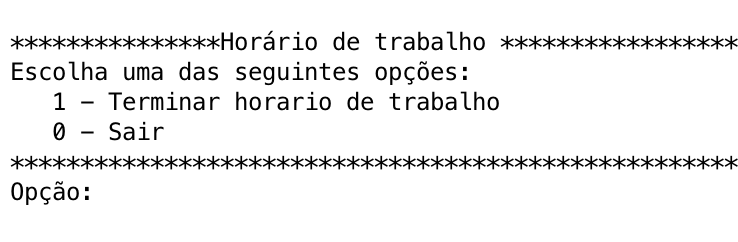
\includegraphics[scale=0.55]{imagem/gerirHorarioTrabalho}
	\small{Menu do motorista para iniciar horario de trabalho}
\end{minipage} 
\hfill
\begin{minipage}[b]{.4\textwidth}
	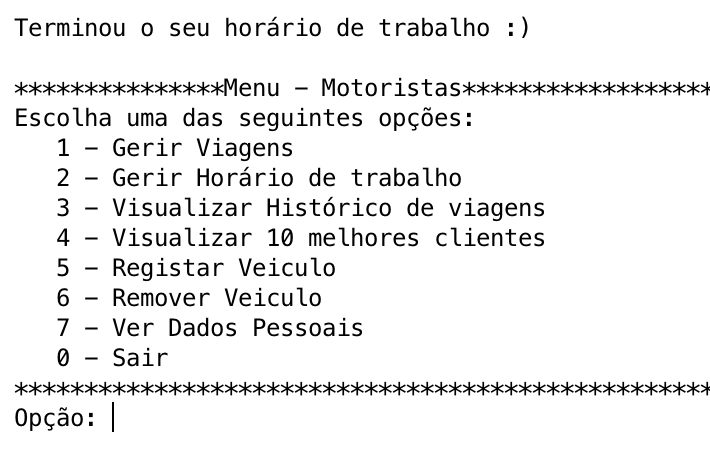
\includegraphics[scale=0.5]{imagem/terminouHorarioTrabalho}
	\small{Menu após terminar horário}
\end{minipage}
\hfill

\newpage

Após terminar o horário, os menus mudam de modo a que o motorista possa voltar ao trabalho, sendo criados para tal os seguintes menus: 

\noindent\begin{minipage}[b]{.4\textwidth}
	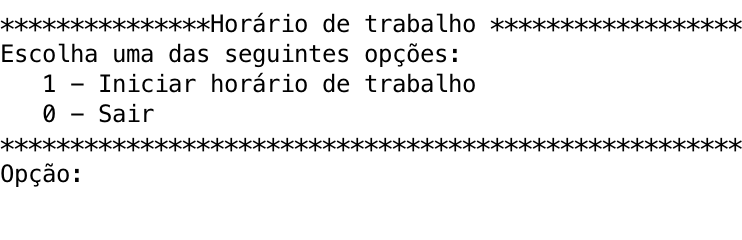
\includegraphics[scale=0.55]{imagem/iniciarHorarioTrabalho}
	\small{Menu do motorista para terminar horario de trabalho}
\end{minipage} 
\hfill
\begin{minipage}[b]{.4\textwidth}
	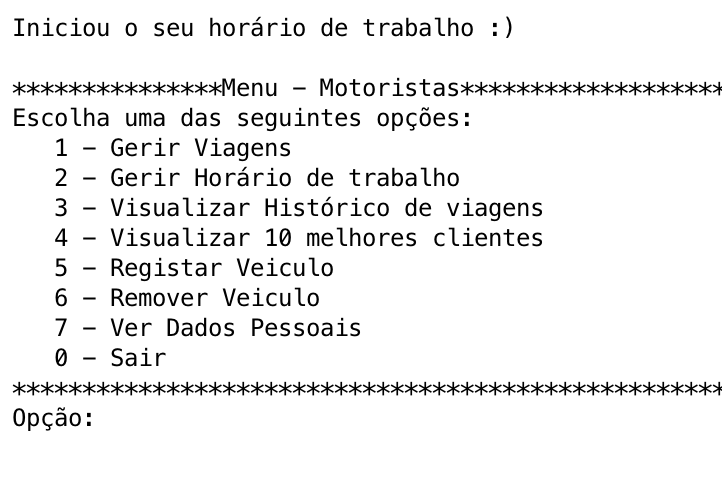
\includegraphics[scale=0.5]{imagem/iniciouHorarioTrabalho}
	\small{Menu após iniciar horário de trabalho}
\end{minipage}
\hfill

\item \textbf{Visualizar Histórico de Viagens}

O menu Visualizar Histórico de viagens permite ao motorista escolher em que tipo de formato prefere ver o histórico ou entre datas ou o total. 
\begin{figure}[htpb]
	\centering
	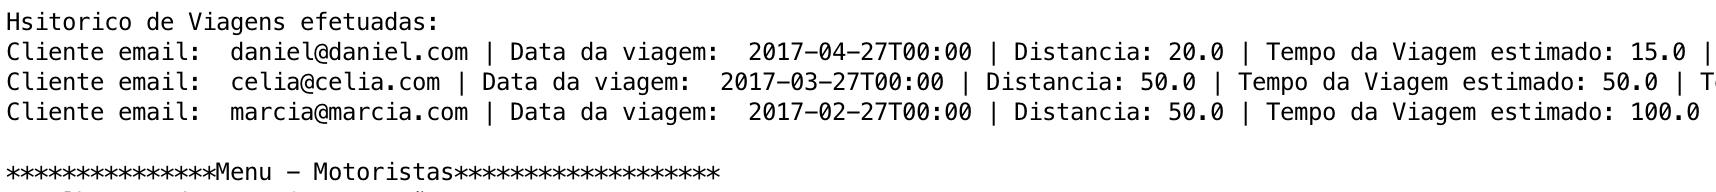
\includegraphics[scale=0.6]{imagem/verViagensMotorista}
	\caption{Menu de visualização de Histórico de viagens}
	\label{p3:fig:p3_verViagensMotorista}
\end{figure}


\item \textbf{Visualizar 10 melhores Clientes}

Esta opção permite ao motorista visualizar quais os seus melhores 10 clientes, isto é os clinetes que gastam mais dinheiro em viagens. 

\begin{figure}[htpb]
	\centering
	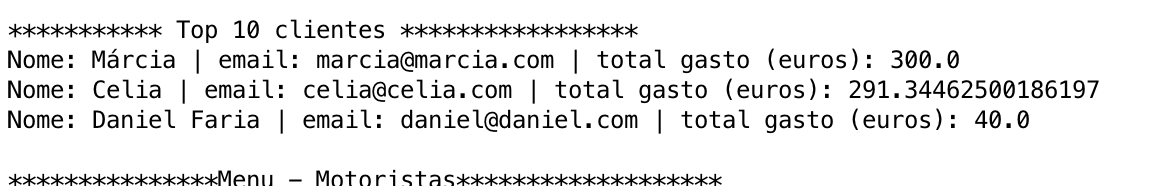
\includegraphics[scale=0.6]{imagem/topClientesMotorista}
	\caption{Menu de visualização de 10 melhores Clientes do Motorista}
	\label{p3:fig:p3_topClientesMotorista}
\end{figure}



\item \textbf{Registar Veiculo}

Esta opção permite ao motorista associar um veiculo a si mesmo. Só é permitido que um um motorista tenha um veiculo associado a si. 

\noindent\begin{minipage}[b]{.4\textwidth}
	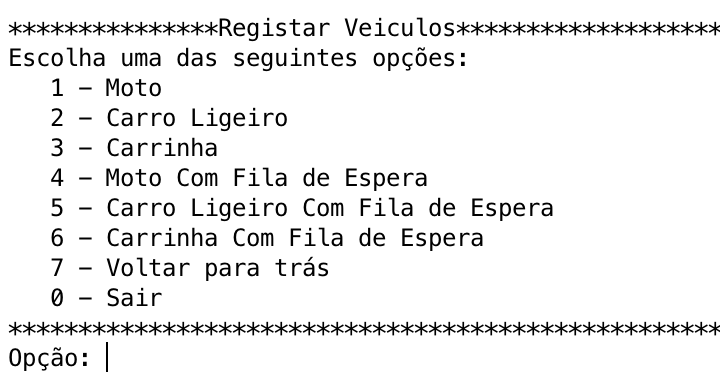
\includegraphics[scale=0.55]{imagem/escolherTipoVeiculo}
	\small{Menu para escolher tipo de veiculo}
\end{minipage} 
\hfill
\begin{minipage}[b]{.4\textwidth}
	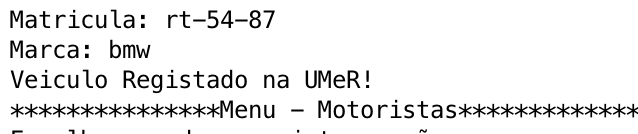
\includegraphics[scale=0.5]{imagem/insercaoDadosVeiculo}
	\small{Menu de inserção de dados no novo veiculo}
\end{minipage}
\hfill


\item \textbf{Remover Veiculo}

Esta opção permite ao motorista remover um veiculo associado a si. 
\begin{figure}[htpb]
	\centering
	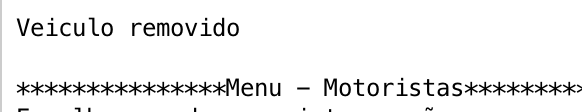
\includegraphics[scale=0.6]{imagem/veiculoRemovido}
	\caption{Menu para remoção do veiculo do motorista}
	\label{p3:fig:p3_veiculoRemovido}
\end{figure}

\end{enumerate}
\subsection{Funcionalidades de Admin}
O Administrador da aplicação tem a funcionalidade principal de visualizar estatísticas, tais como ver uma lista de todos os utilizadores atualizados, os veiculos, o histórico, a lista dos 10 clientes que mais gastam, os motoristas com mais desvios de tempo e custo e ainda poderá ver e editar dados pessoais. 

\begin{figure}[htpb]
	\centering
	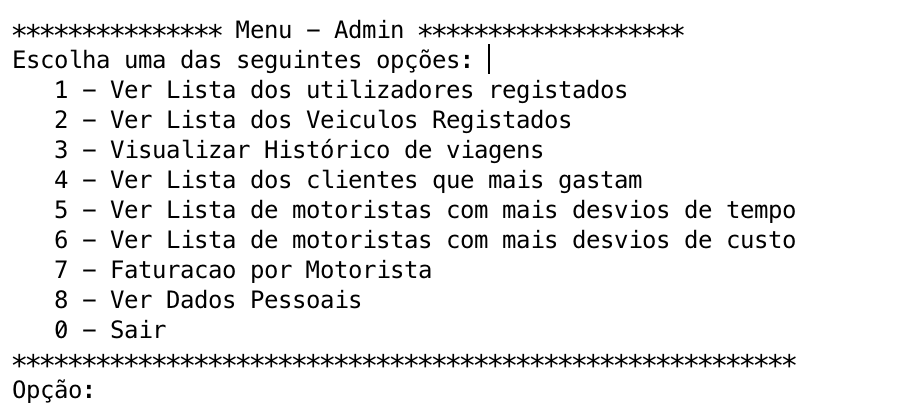
\includegraphics[scale=0.6]{imagem/menuAdmin}
	\caption{Menu do Administrador }
	\label{p3:fig:p3_menuAdmin}
\end{figure}

\newpage
Mostramos de seguida o exemplo de excecução de cada opção do menu: 

\begin{enumerate}
	\item \textbf{Ver lista dos utilizadores Registados}
	\begin{figure}[htpb]
		\centering
		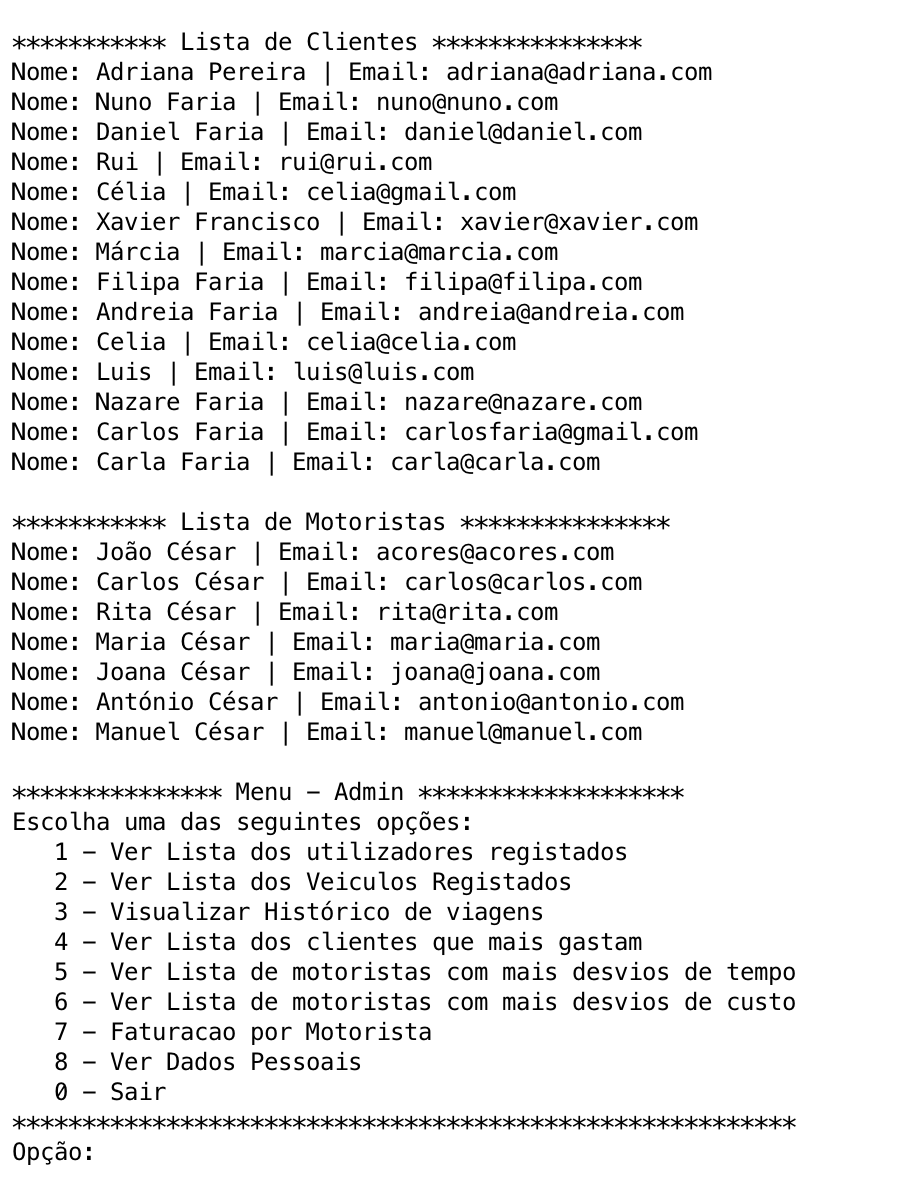
\includegraphics[scale=0.5]{imagem/verListaAtores}
		\caption{Menu do Administrador }
		\label{p3:fig:p3_verListaAtores}
	\end{figure}

\item \textbf{Ver lista dos Veiculos registados }
	\begin{figure}[htpb]
	\centering
	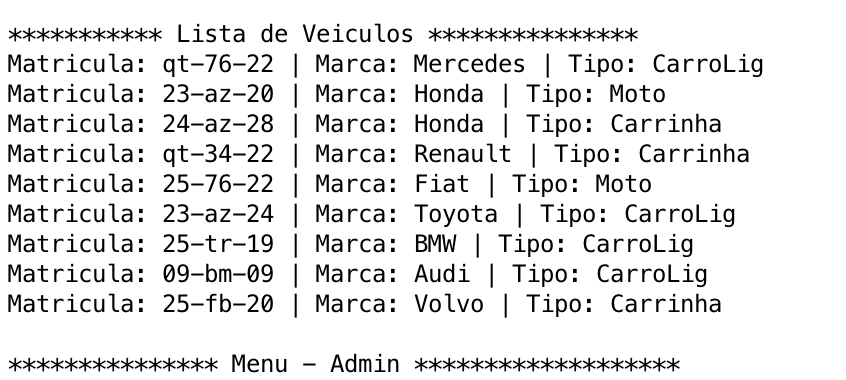
\includegraphics[scale=0.5]{imagem/verListaVeiculos}
	\caption{Ver lista dos veiculos registados }
	\label{p3:fig:p3_verListaVeiculos}
\end{figure}

\newpage
\item \textbf{Visualizar histórico de viagens }

Neste menu o Administrador poderá visualizar todo o histórico ou escolher entre datas, neste caso mostramos como funciona entre datas: 
\begin{figure}[htpb]
	\centering
	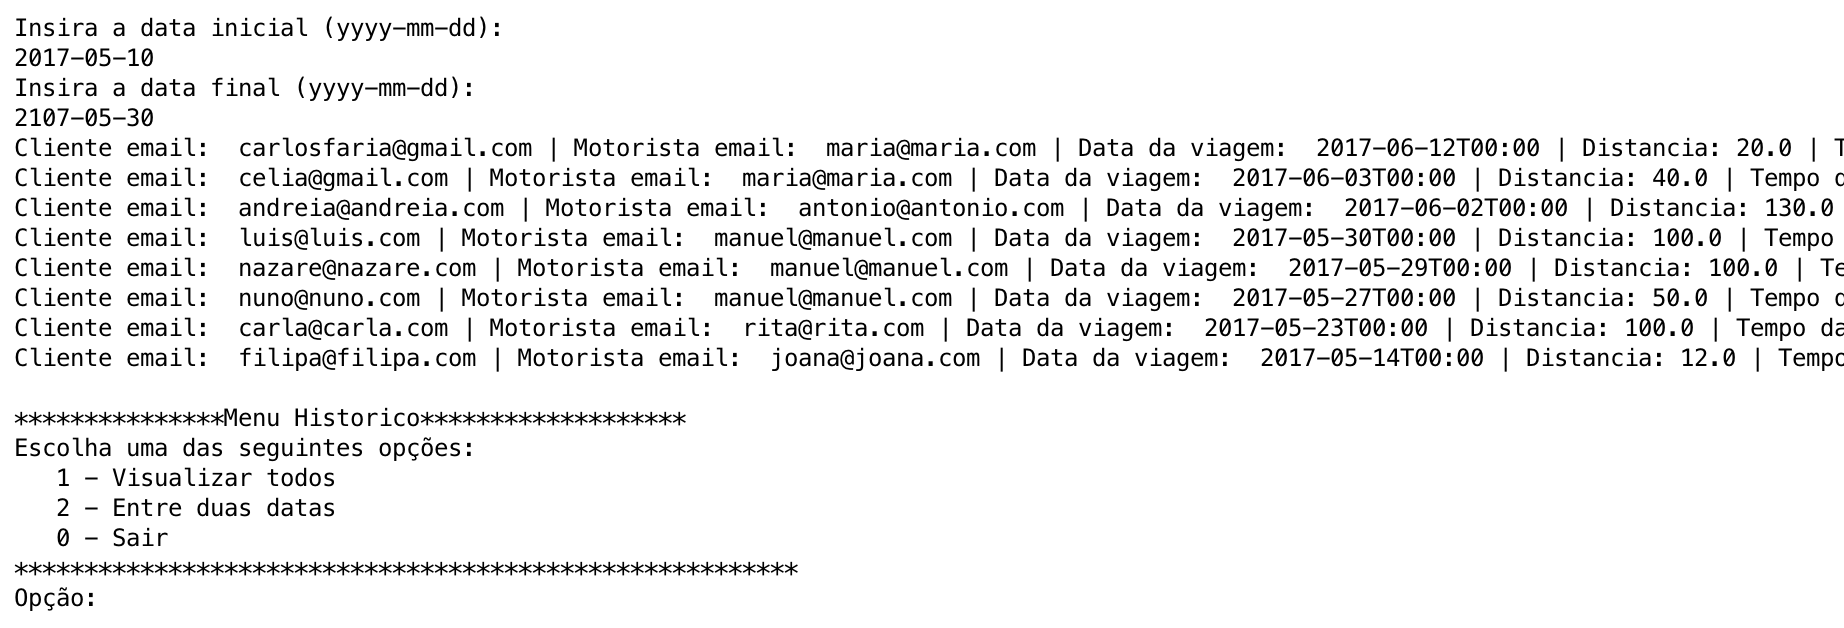
\includegraphics[scale=0.5]{imagem/verListaHistorico}
	\caption{Ver lista de histórico de viagens }
	\label{p3:fig:p3_verListaHistorico}
\end{figure}

\item \textbf{Ver lista dos 10 clientes que mais gastam }

Esta funcionalidade permite listar o top dos 10 melhores clientes da aplicação. 
Este top é construido com base nos históricos terminados (viagens em precurso não são contabilizados para este cálculo). 

\begin{figure}[htpb]
	\centering
	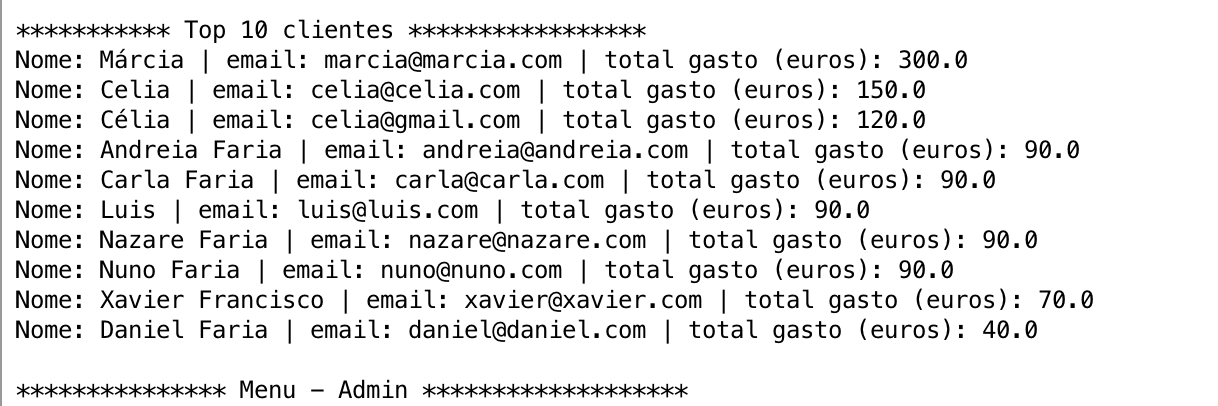
\includegraphics[scale=0.5]{imagem/verClientesMaisGastam}
	\caption{Ver  lista dos 10 clientes que mais gastam  }
	\label{p3:fig:p3_verClientesMaisGastam}
\end{figure}

\item \textbf{Ver lista de motoristas com mais desvios de tempo }

A lista apresentada é ordenada por ordem crescente do grau de cumprimento de tempo. Este valor é calculado com base nos históricos (terminados). Para cada histórico se o tempo estimado for maior que o tempo real, o grau será 100, se o tempo estimado for menor que o tempo real o grau é calculado pela divisão entre o tempo real e o tempo estimado. O grau de cumprimento por motorista é a média do grau de cumprimento dos seus históricos.  

Quanto maior o grau de cumprimento de tempo, melhor será para o cliente uma vez que este grau indica que o motorista efetua viagens com um tempo menor ou igual daquele que foi estimado. 

Para o administradores da plataforma quanto menor o grau de cumprimento de tempo pior uma vez que as viagens demoraram mais tempo do que o estimado e por consequência possibilitará a realização de mesnos viagens (menos faturação). 

\begin{figure}[htpb]
	\centering
	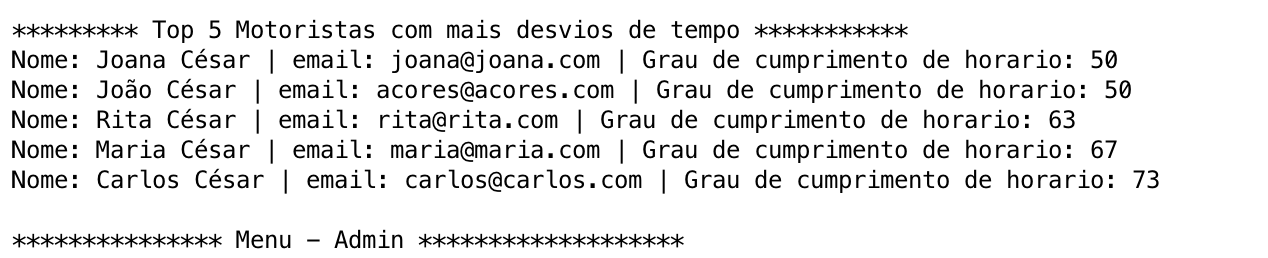
\includegraphics[scale=0.5]{imagem/verMotoristasMaisDesvioTempo}
	\caption{Ver lista de motoristas com mais desvios de tempo }
	\label{p3:fig:p3_verMotoristasMaisDesvioTempo}
\end{figure}

\newpage
\item \textbf{Ver lista de motoristas com mais desvios de custo }

A lista apresentada é ordenada por ordem crescente do grau de cumprimento de custo. Este valor é calculado com base nos históricos (terminados). Para cada histórico se o custo real for maior que o custo estimado, o grau será 100, se o custo real for menor que o custo estimado o grau é calculado pela divisão entre o custo real  e o custo estimado. O grau de cumprimento por motorista é a média do grau de cumprimento dos seus históricos.  

Quanto menor o grau de cumprimento de custo, melhor será para o cliente uma vez que este grau indica que o motorista efetua viagens com um custo menor do que aquele que foi estimado. 

Para o administradores da plataforma quanto menor o grau de cumprimento de custo pior uma vez que as receitas serão menores em relação às receitas estimadas. 


\begin{figure}[htpb]
	\centering
	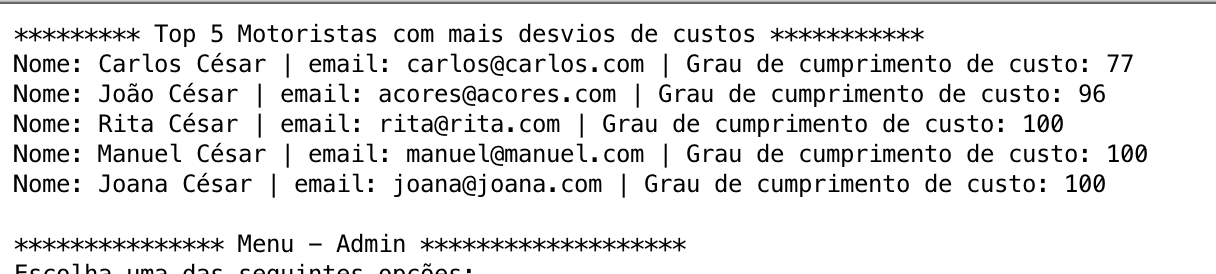
\includegraphics[scale=0.5]{imagem/verMotoristasMaisDesvioCusto}
	\caption{Ver lista de motoristas com mais desvios de custos}
	\label{p3:fig:p3_verMotoristasMaisDesvioCusto}
\end{figure}

\item\textbf{ Faturação por Motorista}

Esta funcionalidade permite ver os dados entre datas ou a lista com todos os dados. Decidiu-se que faria mais sentido apresentar a faturação por motorista, visto que o motorista só tem um veiculo então a informação seria a mesma. 

\begin{figure}[htpb]
	\centering
	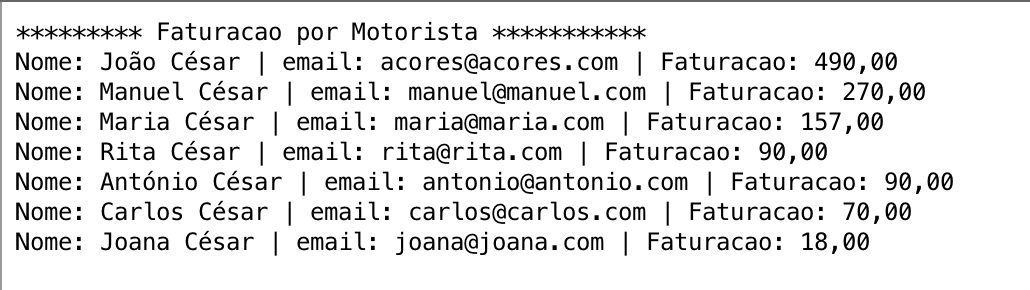
\includegraphics[scale=0.5]{imagem/faturacaoPorMotorista}
	\caption{Ver faturação por motorista}
	\label{p3:fig:p3_faturacaoPorMotorista}
\end{figure}

	
\end{enumerate}


\chapter{Conclusões e }

Aspetos a melhorar seriam a apresentação dos menus, poder-se-ia ter melhorado a organização, assim como o 

listar as funcionalidades ..... 
. as funcionalidade básicas da aplicação que foram implementadas 
existem fatores de aleatoriedade implemnetados para calcular o tempo real 
as filas de espera dos veiculos não podem ser utilizadas, 
não é possivel registar empresas. 
os menus poderiam ter uma melhor organização por exemplos as estaticias que são acedidas pelo admin devia ter um menu de introdução de estatisticas 

os motoristas deveriam poder criar vários veiculos e fazer a gestão do veiculo que estão a utilizar no momento. neste momento o motorista para reutilizar o veículo tem de o voltar a registar 

+/-não podem existir atores de tipos diferentes com o memso email, 

o admin deveria poder gerir clientes motoristas e veiculos 
neste momento só existe um admin e não tem a possibilidade de inserir outros admins 

não foi possivel u

Trabalho Futuro

Permitir registo de empresas e a utilização das filas de espera dos veiculos, para o primeiro ter-se-ia de adicionar um novo tipo de utilizador e dar-lhe permissão para conseguir gerir os seus motoristas e veiculos 

para o segundo seria necessário alterar a requisição de um motorista e  se ele permitisse fila de espera adicionar o cliente a essa fila e alterar o estado do cliente para em fila de espera. 

o admin deveria poder gerir clientes motoristas e veiculos





\end {document}


